\documentclass[a4]{article}

\usepackage[left=2.5cm,right=2.5cm,top=2cm,bottom=2cm]{geometry} 

\usepackage[utf8]{inputenc}   % otra alternativa para los caracteres acentuados y la "ñ"
\usepackage[           spanish % para poder usar el español
                      ,es-tabla % para los captions de las tablas
                       ]{babel}   
\decimalpoint %para usar el punto decimal en vez de coma para los números con decimales

\usepackage[T1]{fontenc}
\usepackage{lmodern}

\usepackage{parskip}
\usepackage{xcolor}

\usepackage{caption}

\usepackage{enumerate} % paquete para poder personalizar fácilmente la apariencia de las listas enumerativas

\usepackage{graphicx} % figuras
\usepackage{subfigure} % subfiguras

\usepackage{amsfonts}
\usepackage{amsmath}

\definecolor{gris}{RGB}{220,220,220}
	
\usepackage{float} % para controlar la situación de los entornos flotantes

\restylefloat{figure}
\restylefloat{table} 

\newcommand{\HRule}{\rule{\linewidth}{0.5mm}}

\author{David Cabezas Berrido}
\date{\vspace{-5mm}}

\title{\huge Aprendizaje Automático: Práctica 2 \HRule\vspace{-4mm}}

\begin{document}
\maketitle
\tableofcontents

\newpage

\section{Ejercicio sobre la complejidad de H y el ruido}

\subsection{Dibujar nubes de puntos}

Utilizando las funciones \texttt{simula\_unif} y \texttt{simula\_gaus},
he generado dos muestras en dimensión 2, de tamaño $N=50$. \\
La primera muestra es una uniforme en el cuadrado
$[-50,50]\times[-50,50]$ 
y la segunda muestra es una normal de media $(0,0)$ y varianza $(5,7)$ 
(desviación típica $(\sqrt{5},\sqrt{7})$). \\
He mantenido fija la escala de los ejes para que se aprecie que los puntos
generados por la normal están mucho más concentrados en torno al punto $(0,0)$,
la concentración es ligeramente mayor en el eje de abscisas 
debido a que tiene menor varianza, pero apenas se aprecia.

\vspace{-3mm}
\begin{figure}[H]
    \centering
    \subfigure[$U\big((-50,50)\times(-50,50)\big)$]{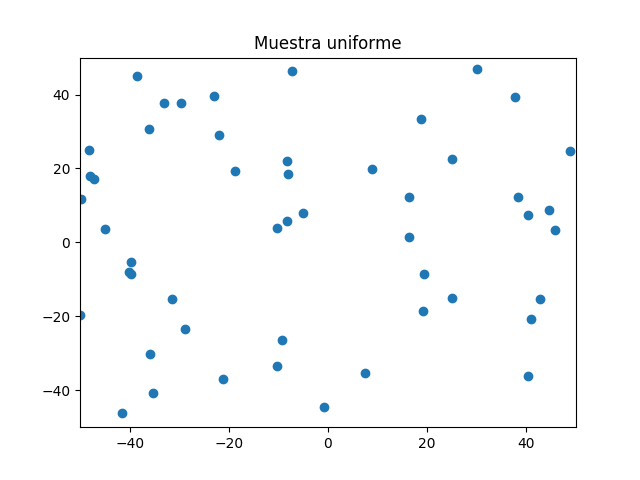
\includegraphics[width=80mm]{imgs/uniform.png}}
    \subfigure[$N\big((0,0),(\sqrt{5},\sqrt{7})\big)$]{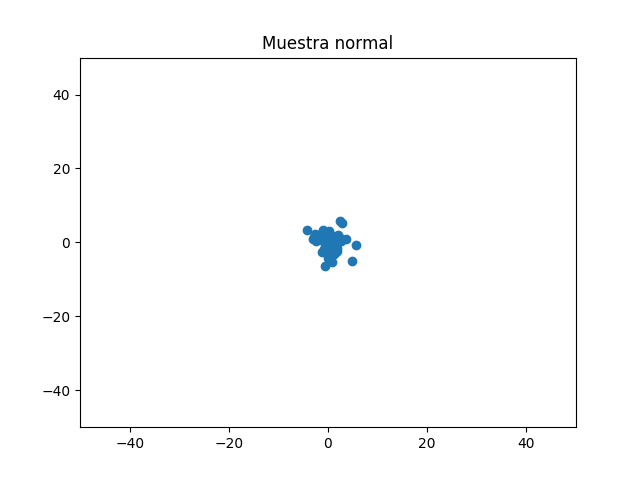
\includegraphics[width=80mm]{imgs/normal.png}}
    \caption{Muestras uniforme y normal}
    \label{fig:uniform-normal}
\end{figure}
\vspace{-6mm}

\subsection{Muestra etiquetada por una recta}

He generado (con \texttt{simula\_unif}) una muestra de $N=100$ puntos
del cuadrado $[-50,50]\times[-50,50]$ y los he etiquetado con
el signo de la distancia a una recta generada por \texttt{simula\_recta} que corta a dicho cuadrado.
Esto quiere decir que si la recta es $y=ax+b$, la etiqueta
de un punto $(x,y)$ es el signo de la función $y-ax-b$ (+1 si el punto 
queda por encima de la recta y -1 si queda por debajo).
Obviamente la recta clasifica a la perfección todos los puntos.

A continuación, he añadido ruido a las etiquetas de la muestra
(10\% en cada clase). Claramente la recta tiene un 10\% de puntos mal clasificados ahora.

\vspace{-2mm}

\begin{figure}[H]
    \centering
    \subfigure[Muestra sin ruido]{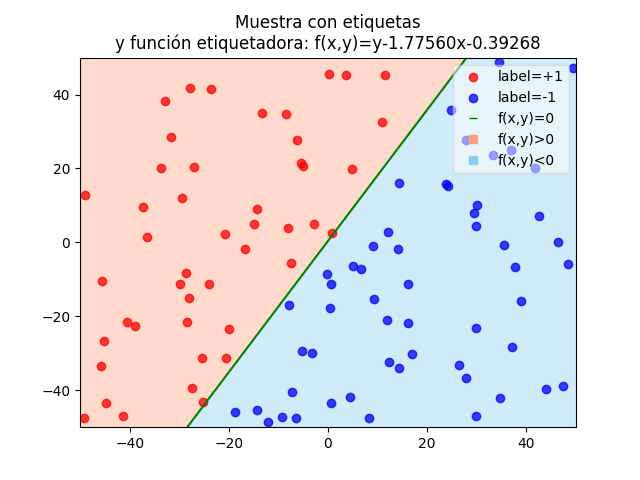
\includegraphics[width=80mm]{imgs/x-f.png}}
    \subfigure[Muestra con ruido]{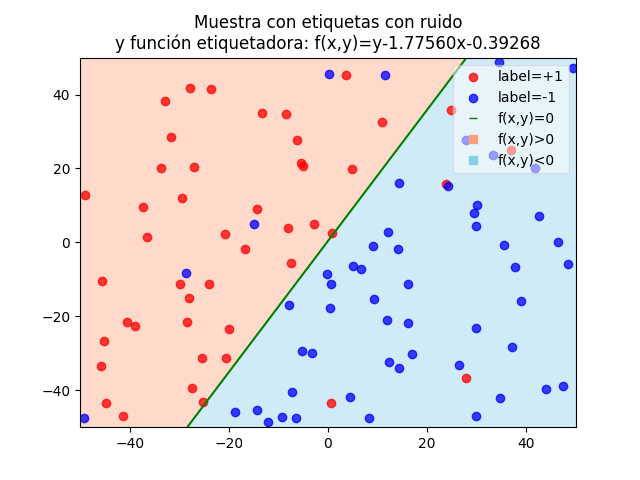
\includegraphics[width=80mm]{imgs/x-f_noise.png}}
    \caption{Muestra y recta etiquetadora}
    \label{fig:muestra-ruido}
\end{figure}

\subsection{Comparación con otras funciones frontera}

Ahora he representado la misma muestra (con ruido) junto con otras funciones,
he calculado también el error que cometen dichas funciones funciones a
la hora de clasificar la muestra.

En la siguiente figura se ve que puntos clasifica bien y mal
cada función, los bien clasificados son los que están en la región de su color.
Incluyo también el porcentaje de puntos mal clasificados para cada función.

\vspace{-3mm}

\begin{figure}[H]
    \centering
    
    \subfigure[$f(x,y)=(x-10)^2+(y-20)^2-400$;\ \ Error: 58\%]{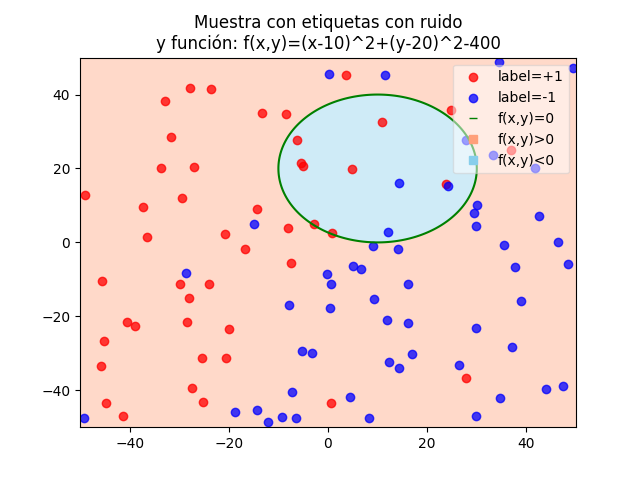
\includegraphics[width=82mm]{imgs/x-f1_noise.png}}
    \subfigure[$f(x,y)=0.5(x+10)^2+(y-20)^2-400$;\ \ Error: 68\%]{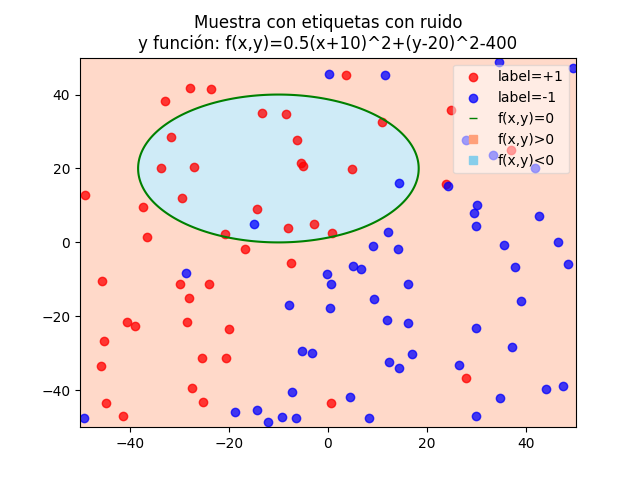
\includegraphics[width=82mm]{imgs/x-f2_noise.png}}
    
    \subfigure[$f(x,y)=0.5(x-10)^2-(y+20)^2-400$;\ \ Error: 35\%]{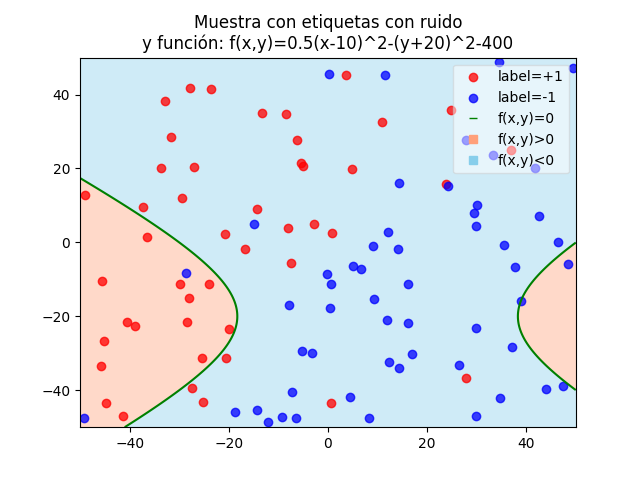
\includegraphics[width=82mm]{imgs/x-f3_noise.png}}
    \subfigure[$f(x,y)=y-20x^2-5x+3$;\ \ Error: 47\%]{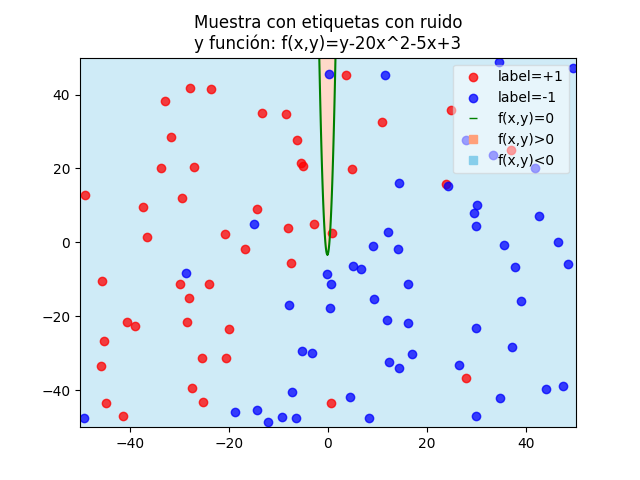
\includegraphics[width=82mm]{imgs/x-f4_noise.png}}
    
    \caption{Muestra con otras funciones como delimitadores}
    \label{fig:muestra-otras}
\end{figure}

\vspace{-3mm}

Ninguna de estas cuatro funciones ha conseguido si quiera acercarse
al error del 10\% que presentaba la recta. Esto era de esperar,
ya que la recta la he usado para etiquetar la muestra (salvo ese 10\% de ruido)
y las funciones estaban prefijadas antes (no han recibido ningún aprendizaje ni ajuste).

Sin embargo, es perfectamente posible que el ruido de la muestra
provoque que el mejor ajuste no sea la misma recta que usé
para etiquetarla, en este caso se puede producir sobreajuste
si la clase H es lo suficientemente compleja como para ajustar el
ruido.

Por ejemplo, si ajustase la muestra sin ruido mediante
una parábola $y=ax^2+bx+c$ el peso $a$ obtendría un valor muy cercano a 0.
Pero en la muestra con ruido, esto puede no ocurrir, es probable
que el valor que se obtenga para $a$ al ajustar la muestra con
ruido no sea cercano a 0, lo que ajustaría mejor la muestra (con ruido)
pero se alejaría de la función objetivo, dando lugar a sobreajuste.

\section{Modelos lineales}

\subsection{Algoritmo Perceptron}

\title{\bf \large Caso de muestra separable:}

He ejecutado el algoritmo PLA sobre la muestra etiquetada del 
ejercicio $2a)$ de la sección anterior y he anotado el número de
iteraciones necesarias para que el algoritmo converja en 10
ejecuciones.

Partiendo del vector 0, en las 10 ejecuciones ha necesitado 2
iteraciones, ya que al partir del mismo punto el comportamiento del
algoritmo es exactamente el mismo. La solución obtenida ha sido
$w=[-3,-57.36159336,28.53120771]$.

\vspace{-3mm}
\begin{figure}[H]
    \centering
    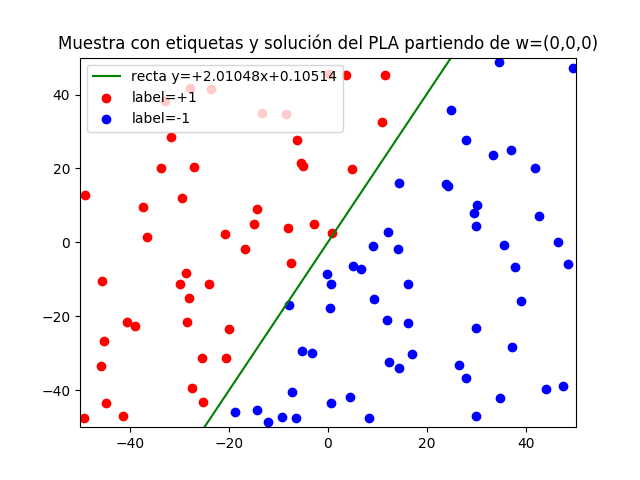
\includegraphics[width=82mm]{imgs/PLA.png}
    \caption{Recta obtenida con PLA partiendo de pesos nulos (muestra separable)}
    \label{fig:PLA}
\end{figure}
\vspace{-3mm}

Luego he realizado 10 ejecuciones partiendo de vectores de números
aleatorios en $[0,1]$, las iteraciones necesarias en cada ejecución
han sido: 2, 3, 3, 2, 3, 2, 3, 2, 3, 3 (media 2.6). Ahora el algoritmo
ha tenido comportamientos diferentes, ya que ha partido de un $w_{ini}$
diferente en cada iteración.
En este caso el número de iteraciones no presenta más que una ligera
variación respecto al vector inicial, pero con muestras (variando la
semilla) he obtenido resultados muy variados (tanto mejores como peores),
luego no podemos concluir nada respecto a la eficiencia del algoritmo.

\title{\bf \large Caso de muestra no separable:}

He realizado el mismo experimento con la muestra etiquetada del
ejercicio $2b)$ de la sección anterior, que es la misma muestra pero
con ruido en las etiquetas, este ruido hace que los datos no sean 
separables y que el algoritmo no converja. He limitado las iteraciones
a 500 para que pare en algún momento y efectivamente ha agotado las
500 iteraciones en todos los casos, tanto partiendo del vector cero
como de vectores de valores aleatorios en $[0,1]$. Partiendo del 
vector cero, he obtenido la solución $w=[-45,-37.98579548,38.22893039]$.

\vspace{-3mm}
\begin{figure}[H]
    \centering
    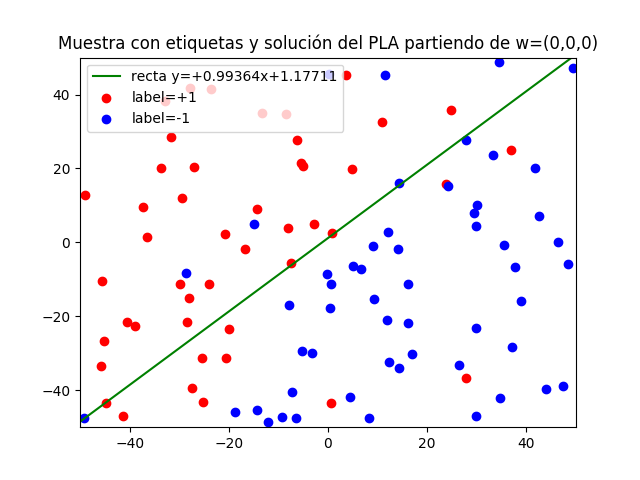
\includegraphics[width=82mm]{imgs/PLA_noise.png}
    \caption{Recta obtenida con PLA partiendo de pesos nulos (muestra no separable)}
    \label{fig:PLA}
\end{figure}
\vspace{-3mm}

\subsection{Regresión Logística}



\section{Bonus: Clasificación de dígitos}

%%%% Describir problema de clasificación binaria

Primero he ajustado un modelo de Regresión Lineal, usando el algoritmo
de la pseudoinversa. \\ He obtenido los pesos $w= [-0.50676351,  8.25119739,  0.44464113]$
 y los errores de clasificación (proporción de puntos mal clasificados) $E_{in}=0.22780569514237856$ y $E_{test} = 0.25136612021857924$.

\begin{figure}[H]
    \centering
    \subfigure[Resultado regresión junto con datos de entrenamiento]{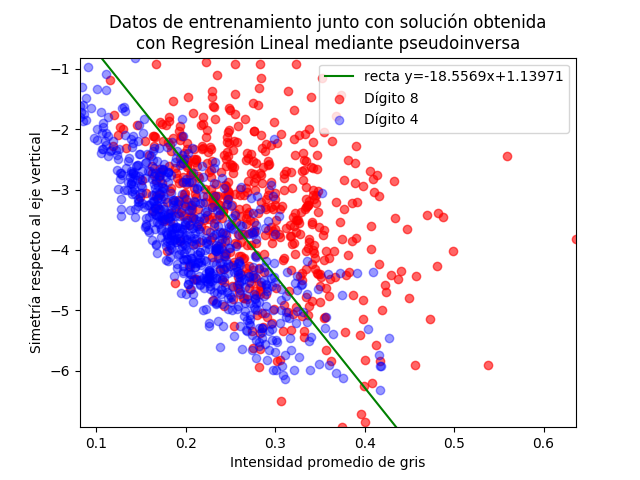
\includegraphics[width=82mm]{imgs/lin-regress.png}}
    \subfigure[Resultado regresión junto con datos de test]{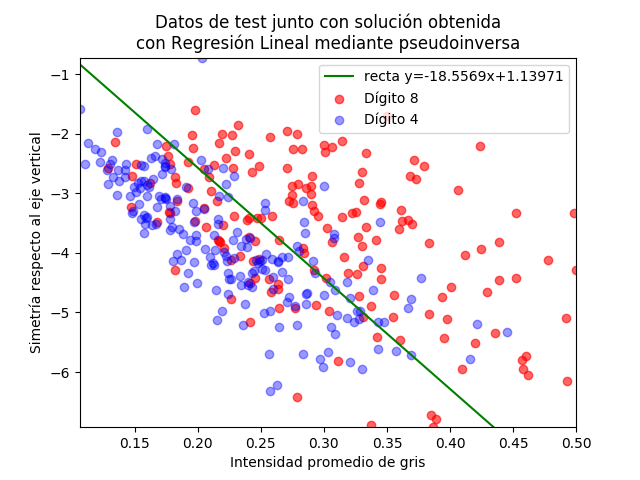
\includegraphics[width=82mm]{imgs/lin-regress_test.png}}
    \caption{Recta obtenida por Regresión Lineal con pseudoinversa}
    \label{fig:lin-regress}
\end{figure}
\vspace{-3mm}

A continuación, he utilizado esa solución como valor inicial para
el algoritmo PLA-Pocket con 100 etapas, he obtenido los pesos $w= [-6.50676351, 94.33278003, 4.88432863]$
y los errores de clasificación (proporción de puntos mal clasificados)
$E_{in} = 0.22529313232830822$ y $E_{test} = 0.2540983606557377$.

\begin{figure}[H]
    \centering
    \subfigure[Resultado PLA-Pocket junto con datos de entrenamiento]{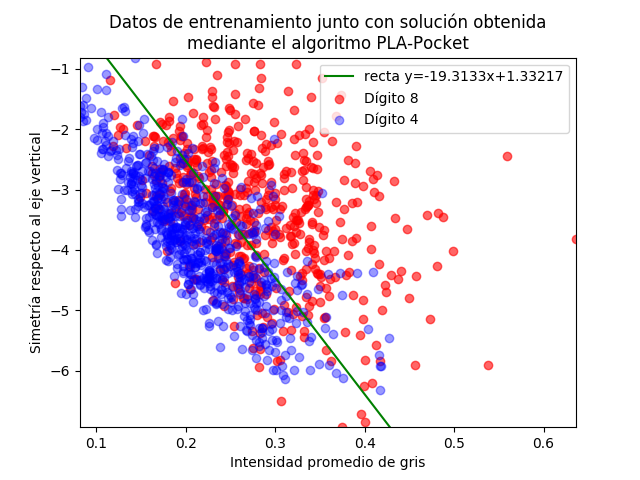
\includegraphics[width=82mm]{imgs/PLA-pocket.png}}
    \subfigure[Resultado PLA-Pocket junto con datos de test]{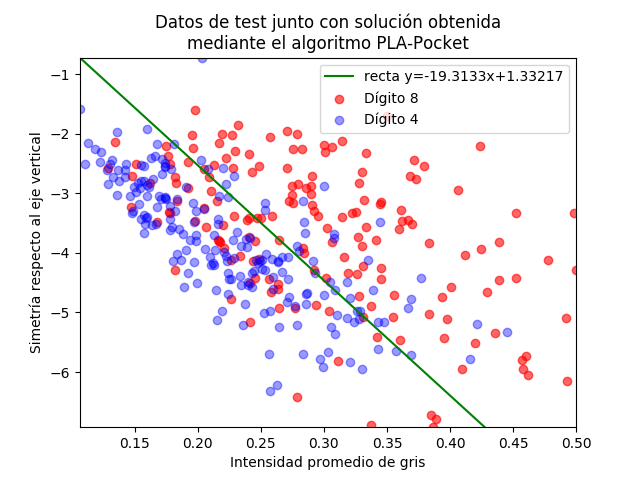
\includegraphics[width=82mm]{imgs/PLA-pocket_test.png}}
    \caption{Recta obtenida con PLA-Pocket}
    \label{fig:lin-regress}
\end{figure}
\vspace{-3mm}

Obviamente en PLA-Pocket $E_{in}$ no puede empeorar respecto al inicial,
he obtenido un $E_{in}$ ligeramente más bajo y $E_{test}$ ligeramente más alto 
al aplicar la mejora de PLA-Pocket.


\end{document}

% REVISAR
Utilizando la fórmula
\[E_{out}(h)\leq E_{in}(h)+\sqrt{\frac{1}{2N}\log{\frac{2}{\delta}}}\qquad\text{con probabilidad}\geq 1-\delta\]
puedo calcular una cota para $E_{out}$ basada en $E_{in}$ con tolerancia $0.05$.
En el conjunto de entrenamiento $N=1194$. Luego puedo asegurar con probabilidad mayor o igual que 0.95 que
\[E_{out}\leq 0.22529313232830822 + \sqrt{\frac{1}{2388}\log{\frac{2}{\delta}}}=0.22529313232830822+0.0393033954=0.2645965277\]

\end{document}